%!TEX TS-program = xelatex
\documentclass[12pt,a4paper]{article}
\usepackage{fontspec}
\setmainfont{Times New Roman}
\setmonofont{Consolas}
\usepackage[russian]{babel}
\usepackage[left=25mm,right=15mm,top=20mm,bottom=20mm]{geometry}
\usepackage{amsmath,array,booktabs,listings,graphicx}
\setlength{\parindent}{1.25cm}
\setlength{\parskip}{3pt}
\setlength{\emergencystretch}{3em}
\pagestyle{plain}
\lstset{basicstyle=\ttfamily\fontsize{9}{11}\selectfont,
 columns=fullflexible,keepspaces=true,breaklines=true,
 numbers=none,tabsize=4,showstringspaces=false,
 frame=single,xleftmargin=0pt,
 aboveskip=5pt,belowskip=5pt}

\begin{document}
\section*{1 Цель работы}
Изучить цепочечные команды и приобрести практические навыки их применения
для обработки строк символов.

\section*{2 Постановка задачи}
Написать программу на языке ассемблера, которая по исходной строке
формирует палиндром, используя цепочечные команды.

Способ построения: к исходной строке $S$ дописывается её обратная запись
$S^R$. Результат $P=S\,S^R$ одинаково читается в обоих направлениях.
Например, \texttt{abcd} преобразуется в \texttt{abcddcba}.

Программа предназначена для 32-разрядной Windows и собирается MASM.
Вводится строка длиной до 255 символов в однобайтовой кодировке CP866,
включая русские буквы. Пробелы, регистр и знаки препинания сохраняются.
Пустая строка даёт пустой результат; слишком длинный ввод отклоняется.

\section*{3 Алгоритм}
\begin{enumerate}
\item Получить дескрипторы консоли и прочитать исходную строку функцией
\texttt{ReadConsoleA}. Проверить длину ввода. Не учитывать завершающие
символы CR и LF; обозначить длину исходной строки через $n$.
\item Сбросить флаг направления командой \texttt{CLD}. Поместить адреса
исходного и результирующего буферов в \texttt{ESI} и \texttt{EDI},
а $n$ в \texttt{ECX}. Скопировать строку командой \texttt{REP MOVSB}.
\item Если $n=0$, перейти к выводу. Иначе установить \texttt{ESI} на
последний символ исходной строки и выполнить $n$ повторений:
\texttt{STD; LODSB; CLD; STOSB}.
\texttt{LODSB} читает символ в \texttt{AL} и уменьшает \texttt{ESI},
а \texttt{STOSB} записывает символ и увеличивает \texttt{EDI}.
\item Добавить CR и LF в конец результата. Вывести $2n+2$ байта
функцией \texttt{WriteConsoleA} и завершить программу.
\end{enumerate}

\newpage
\section*{4 Используемые команды и функции}
\begin{itemize}
\item \texttt{REP MOVSB} --- копирование $n$ байт из \texttt{[ESI]}
в \texttt{[EDI]}, счётчик повторений --- \texttt{ECX}.
\item \texttt{STD}, \texttt{CLD} --- выбор направления движения указателей;
\texttt{LODSB}, \texttt{STOSB} --- чтение байта в \texttt{AL} и запись
байта из \texttt{AL}.
\item \texttt{GetStdHandle}, \texttt{ReadConsoleA}, \texttt{WriteConsoleA}
--- получение дескрипторов, ввод и вывод; \texttt{ExitProcess} --- завершение.
\item \texttt{SetConsoleCP}, \texttt{SetConsoleOutputCP} --- установка CP866;
\texttt{PrintText} --- вывод заданного количества байтов.
\end{itemize}

\section*{5 Тестирование}
Результаты проверки приведены в таблице. Проверены строки разной длины,
пробелы, русские буквы и превышение допустимой длины ввода.
Во всех случаях результат совпал с ожидаемым.

В таблице $\varepsilon$ обозначает пустую строку, $\sqcup$ --- пробел,
а степень --- число повторений строки.

\begin{center}
\small
\renewcommand{\arraystretch}{1.22}
\begin{tabular}{@{}c p{37mm} p{66mm} c@{}}
\toprule
№ & Исходная строка & Фактический результат & Код выхода \\
\midrule
1 & $\varepsilon$ & $\varepsilon$ & 0 \\
2 & \texttt{a} & \texttt{aa} & 0 \\
3 & \texttt{ab} & \texttt{abba} & 0 \\
4 & \texttt{abc} & \texttt{abccba} & 0 \\
5 & \texttt{abcd} & \texttt{abcddcba} & 0 \\
6 & \texttt{aba} & \texttt{abaaba} & 0 \\
7 & \texttt{aaaa} & \texttt{aaaaaaaa} & 0 \\
8 & \texttt{a b} & \texttt{a bb a} & 0 \\
9 & $\sqcup a\sqcup$ & $\sqcup a\sqcup\sqcup a\sqcup$ & 0 \\
10 & \texttt{Ab1!} & \texttt{Ab1!!1bA} & 0 \\
11 & \texttt{тест} & \texttt{тесттсет} & 0 \\
12 & \texttt{а роза} & \texttt{а розаазор а} & 0 \\
13 & $(\texttt{abc})^{85}$, 255 символов
   & $(\texttt{abc})^{85}(\texttt{cba})^{85}$, 510 символов & 0 \\
14 & $\texttt{a}^{256}$ & Ошибка: превышена длина ввода & 1 \\
15 & $\texttt{b}^{300}$ & Ошибка: превышена длина ввода & 1 \\
\bottomrule
\end{tabular}
\end{center}

\newpage
\noindent\textbf{Скриншоты консоли Windows}\\
Ниже приведены снимки окон консоли при выполнении двух тестов.

\medskip
\noindent\textbf{Тест № 11}\\
Назначение: обработка русских букв в CP866.\\
Ожидается: \texttt{тесттсет}, код завершения 0.
\begin{center}
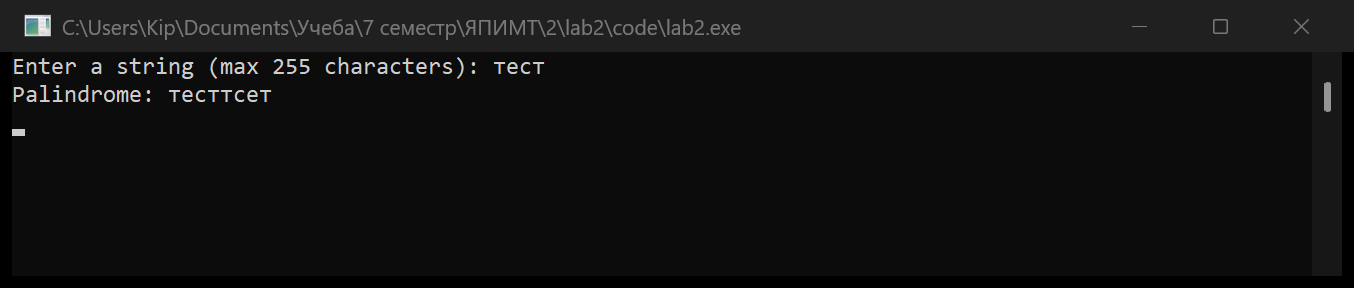
\includegraphics[width=\linewidth]{../tests/screenshots/11-russian.png}
\end{center}

\medskip
\noindent\textbf{Тест № 14}\\
Назначение: отклонение строки из 256 символов \texttt{a}.\\
Ожидается: сообщение об ошибке, код завершения 1.
\begin{center}
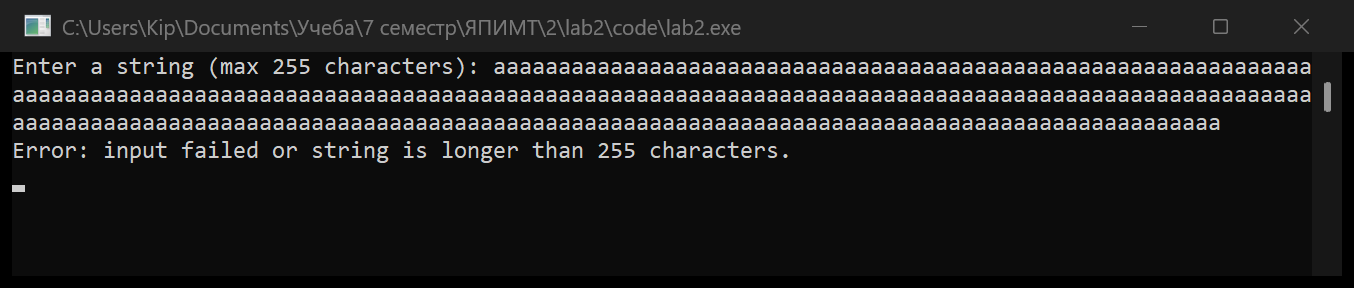
\includegraphics[width=\linewidth]{../tests/screenshots/14-too-long.png}
\end{center}

\section*{6 Код программы}
\lstinputlisting{../code/main.asm}

\section*{7 Вывод}
Палиндром формируется копированием исходной строки командой \texttt{REP MOVSB}
и добавлением её обратной записи с помощью \texttt{LODSB} и \texttt{STOSB}.
Для чтения назад и записи вперёд используются \texttt{STD} и \texttt{CLD}.
Пустая строка обрабатывается без ошибки, а ввод длиннее 255 символов отклоняется.

\end{document}
